%% Template for SDP report, adapted from mlp_cw2_template, 2018. 

%% Based on  LaTeX template for ICML 2017 - example_paper.tex at 
%%  https://2017.icml.cc/Conferences/2017/StyleAuthorInstructions

\documentclass{article}
\usepackage[T1]{fontenc}
\usepackage{amssymb,amsmath}
\usepackage{txfonts}
\usepackage{microtype}
\usepackage{xspace}
\xspaceaddexceptions{\%}

% Lists with less spacing between items
\usepackage{paralist}

% For figures
\usepackage{graphicx}
\usepackage{subfig} 

% For citations
\usepackage{natbib}

% For algorithms
\usepackage{algorithm}
\usepackage{algorithmic}

% the hyperref package is used to produce hyperlinks in the
% resulting PDF.  If this breaks your system, please commend out the
% following usepackage line and replace \usepackage{mlp2017} with
% \usepackage[nohyperref]{mlp2017} below.
\usepackage{hyperref}
\usepackage{url}
\urlstyle{same}

% Packages hyperref and algorithmic misbehave sometimes.  We can fix
% this with the following command.
\newcommand{\theHalgorithm}{\arabic{algorithm}}


% Set up MLP coursework style (based on ICML style)
\usepackage{mlp2018}
\mlptitlerunning{SDP Demo \demoNumber  Group (\groupNumber)}
\bibliographystyle{icml2017}


\DeclareMathOperator{\softmax}{softmax}
\DeclareMathOperator{\sigmoid}{sigmoid}
\DeclareMathOperator{\sgn}{sgn}
\DeclareMathOperator{\relu}{relu}
\DeclareMathOperator{\lrelu}{lrelu}
\DeclareMathOperator{\elu}{elu}
\DeclareMathOperator{\selu}{selu}
\DeclareMathOperator{\maxout}{maxout}







%% You probably do not need to change anything above this comment

%% REPLACE the details in the following commands with your details
\setGroupNumber{15}
\setGroupName{Detroit}
\setProductName{Tadashi}
\setLogoFileName{figs/sdp_logo_placeholder.png}

\begin{document} 

\makeSDPTitle{Project Plan}

% Previous MLP Style Title Layout working. 
% \twocolumn[
    % \mlptitle{\productName: SDP Demo \demoNumber}
    % \centerline{Group \groupNumber: \groupName}
% ]

\begin{abstract}
  We propose an assistive healthcare robot, {\it Tadashi}, to automate simple tasks within a care home or supported living environment and allow caregivers to spend more time caring for their patients.
  {\it Tadashi} will automate three key tasks in the caregiver's day. Firstly, waking a patient up at a time specified by the caregiver, by coming into their room and speaking to them. Secondly, bringing water and food to patients at specified times. Thirdly, checking on the welfare of the patient while the caregiver is occupied elsewhere, by coming to their room and asking the patient if they are okay and if they need a caregiver to attend to them. 
\end{abstract} 

\section{Goal description}
Caregivers are overworked: they spend a large amount of time on menial tasks, limiting the amount of time they can spend caring for patients. Our assistive healthcare robot allows caregivers to automate certain menial and administrative tasks, allowing them to spend less time on the menial work, and more time doing what matters: caring for their patients. 

\subsection{Relevance of the system}
\subsubsection{The problem space}
Tadashi is designed to tackle two problems facing caregivers in assisted living situations:
\begin{enumerate}
\item High caregiver:patient ratios, meaning caregivers have little time to dedicate per patient;
\item High administrative loads on caregivers, meaning they must spend more time on administration and menial tasks and less on caring for their patients directly.
\end{enumerate}

There is no national guidance on staffing levels and caregiver:patient ratios in care homes \cite{rcnstaffingadvice}, but research shows that in care homes there is an average ratio of 18 patients per registered nurse during the day, and 26 patients at night \cite{rcnstaffingguidance}.

With this many patients to take care of, nurses struggle to get the time they need with patients. In a 2017 survey on the impact of high nurse:patient ratios \cite{unison}, 63.2\% of nurses said that comforting or talking to patients was rushed, unfinished, not done to an acceptable standard, or missed entirely.

Equally, a 2013 survey showed that nurses spend almost 1/5 of their day on administrative tasks; and only 20\% are satisfied with how they spend their time --- preferring to spend less time on admin and more time on direct care \cite{rcnpol}.

By automating some tasks using Tadashi, we propose that nurses can decrease the amount of time they spend on administrative tasks, and increase the amount of time they spend caring for patients. 

With elderly populations in particular, hydration and nutrition presents a pressing concern \cite{hydrate}. A Care Quality Commission inspection in 2011 found that three out of 12 NHS trusts inspected failed to meet standards required by law in meeting patient needs regarding nutrition and hydration \cite{cqc}. A 2018 report from the Office for National Statistics found that more than 600 care home residents died suffering from malnutrition or dehydration between 2013 and 2017 \cite{ons}.

The problems mentioned above will only get worse in the future. It is estimated that by 2035, up to 190,000 more people aged 65 years or above will require some level of care, and increase of 86\% from today \cite{lancet}. Meanwhile, ongoing staffing issues in the NHS mean that in 10 years time the NHS will have a shortfall of 108,000 nurses \cite{nuffield}. This combination of factors will drive demand for innovative solutions --- including assistive technology like Tadashi.


\subsubsection{Existing solutions}
The most relevant existing solution to the problems we have identified is the work of Fraunhofer IPA on service robots in residential care facilities. As part of the WiMi-Care project, they implemented and tested Care-O-bot 3, a `robot butler' that tracks residents' hydration and brings them water if they have not drunk enough. The goal of this project was to automate certain service-related tasks in order to relieve pressure on care staff \cite{fraunhofer}.

The key takeaways from this work that we will take into account in our project:
\begin{itemize}
\item Patient feedback to the robot was positive: ``inhabitants  understood  the  idea  of  a  robot  supporting  the  staff  without replacing them and showed no fear to interact with the machine'' \cite{springer}. 
\item Adding speech output to address patients by name helped to improve perceptions of the robot and compliance with drinking the water it offered \cite{ieee}. 
\item Staff reaced positively to the introduction of the robot: ``The overall reaction from the personnel (...) was very positive'' (ibid). 
\end{itemize}

\subsection{High-level description} 
We can describe three key user stories to exemplify the functionality of our solution:
\begin{enumerate}
\item Waking the patient
\item Bringing food or water to the patient
\item Checking on the patient
\end{enumerate}

\subsubsection{Waking the patient}
\begin{enumerate}
\item The caregiver specifies in the app what time each patient should wake up.
\item At the specified time, Tadashi navigates to the specified patient's room.
\item Once in the room, Tadashi speaks to wake the user up. A button is accessible to the patient to press once they have woken up:
  \begin{enumerate} 
  \item If the patient does not press the button, Tadashi sends an alert to the caregiver's app, who can then go check on the person. 
  \end{enumerate}
\item Tadashi returns to his starting spot to await the next command. 
\end{enumerate}

\subsubsection{Bringing food or water to the patient}
\begin{enumerate}
\item The caregiver specifies in the app for each patient:
  \begin{itemize}
  \item The intervals at which they should be brought water (or another drink).
  \item The times at which they should be brought food.
  \end{itemize}
\item At the specified time, Tadashi navigates to the pick-up point for food or water.
\item Tadashi moves to the patient's room and passes over the food or water using its arm.
\item Tadashi returns to his starting spot to await the next command.
\end{enumerate}


\subsubsection{Checking on the patient}
\begin{enumerate}
\item The caregiver specifies in the app that Tadashi should go check on a specified patient. 
\item Tadashi navigates to the specified patient's room.
\item Once in the room, Tadashi speaks to the user and asks if they are okay:
  \begin{enumerate}
  \item A button is accessible to the patient to press to reply yes or no.
  \item If the user presses the okay button, Tadashi informs the caregiver through the app. 
  \item If the user presses the not okay button or does not press a button at all, Tadashi informs the caregiver through the app.
  \end{enumerate}
\item Tadashi returns to his starting spot to await the next command. 
\end{enumerate}

\section{Task planning}

\subsection{Milestones} 
We will split the work of each team into four milestones, each corresponding to a demo date. 

\subsubsection{Milestone 1}

For the first demo on February 5th we plan to present our robot base frame with basic movement and tracking functionality, as well as a skeleton android app.

Robot sub goals:
\begin{itemize}
\item The base frame will be able to rotate on the spot to face a given direction.
\item The chassis is sturdy enough to carry a light load, representing future components.
\item The robot can move around freely by remote control.
\item Attach a mounted colour sensor to track tape on the floor.  
\end{itemize}


Once these sub goals are achieved, our robot base frame will be able to reliably and precisely follow along a straight line path of tape. 

App sub goals:
\begin{itemize}
\item Create a functioning android app which can run on a mobile device.
\item Produce a Database which can store a patient's name and one of their health conditions.
\item Implement GDPR features into the Database.
\item Implement functionality in the App to create and edit patient information in the Database.
\end{itemize}
With these sub goals achieved, we can demonstrate updating the Database from the Android app.

\subsubsection{Milestone 2}

For the second demo on February 26th we will showcase our robot with several new components and movement abilities, plus connectivity and interaction with the android app.  

Movement sub goals:
\begin{itemize}
\item Program the robot to recognise turns in a tape path
\item Implement a memory system that allows the robot to remember it's current state 
\end{itemize}

With these new features, we will demonstrate the robot following along a bending line of tape on the floor, navigating around turns in the path.

Component sub goals:
\begin{itemize}
\item Attach a robotic arm which can later be programmed to perform patient assisting tasks.
\item Equip the base frame with a lift system, which can be used to raise the robot's height in order to interact with patients in hospital beds.
\item Implement external buttons which can be pressed to send a signal.
\end{itemize}

App sub goals:
\begin{itemize}
\item Accessible User Interface.
\item Recieves alerts from the robot when it's button is pressed.
\end{itemize}

\subsubsection{Milestone 3}

On March 11th for the third demo we will present the robot with more freedom of movement as well as camera and app functionality.

Camera sub goals:
\begin{itemize}
\item Mount a camera to the robot
\item Send pictures from the camera to the app
\end{itemize}

With these goals achieved, we aim to demonstrate the robot taking an image and then sending it to the mobile app for verification.

Movement sub goals:
\begin{itemize}
\item Implement functionality to move around between rooms without needing a line of tape to follow.
\end{itemize}
App connectivity sub goals:
\begin{itemize}
\item Direct remote control of movement from the app.
\item App provides arm remote control.
\item The app will recieve photos from the robot and display them to the user for verification.
\end{itemize}

\subsubsection{Milestone 4}

On the final demonstration on March 30th we will show our completed prototype with all components working together

App sub goals:
\begin{itemize}
\item  A timetable will be implemented, allowing the user to plan out which rooms should be visited at which times, to check up on the patients.
\item GPS functionality will be provided, so that the robot can be tracked if it is stolen.
\item Full remote control over the robot via the app.
\end{itemize}

Robot behaviour sub goals:

Feature to avoid bumping into obstacles in it's path

Finally, our robot should be able to present our use case by using full connectivity between the app and it's components to plan out it's movement between rooms and in each room interact approriately with the patient, reporting relevant info back to the app for a user to review.


\subsection{Task Decomposition}

We have split our team into three groups to manage the respective tasks of Robot Building, Robot Coding and App Development. For each Milestone we assigned the sub goals to the relevant team, and also planned how our sub teams will work together to implement these as working features.
For each sub-task we assigned a difficulty rating ranging from simplest to most complex with XS, S, M, L , XL


\subsubsection{Robot Building}

Milestone 1: We will build two early versions of the robot base frame with basic moving functionality in all directions and with a colour sensor mounted for tracking a line of tape. The base should be sturdy and able to hold a light load. 

Sub tasks:

Movement Base Frame
\begin{itemize}
\item Building two frames: One from Lego and one using TurtleBot (M)
\end{itemize}
Testing
\begin{itemize}
\item Testing base frames of Lego vs Turtlebot (L)
\item Metrics: Battery life, turn radius, maximum load, speed
\item Also test for potential customisability
\end{itemize}
    
Colour sensor
    Attaching lego colour sensor underneath the base pointing towards tape on the ground, and wiring this to a lego EV3 brick for the       coding team to use in pathfinding (S)
    
Milestone 2: Main robot components attached

Components:
\begin{itemize}
\item Arm(S)
\item Lift to raise robot(XL)
\item Physical buttons (M)
\end{itemize}
    
Milestone 3: Camera attached and sending a signal(M)

Milestone 4: Robot has all components attached and is sturdy enough to move between rooms and complete tasks according to it's timetable(L) 


\subsubsection{Robot Coding}

Milestone 1: Robot can move around and follow a straight line of tape.

Sub tasks: 

Basic RC of robot:
\begin{itemize}
\item Connecting software to motor controls using ROS and EV3 (S)
\item Moving forward and backwards (S)
\item Rotating on the spot and turning to face a specified direction angle (M)
\end{itemize}
Robot Pathfinding system:
\begin{itemize}
\item Robot can recognise tape underneath it and follow the tape in a straight line (L)
\end{itemize}
Testing:
\begin{itemize}
\item Testing out the ROS programming of Turtlebot vs the Python programming of Lego mindstorms EV3 block to decide which is simplest and most customisable to find the best platform solution on which to build our pathfinding algorithms (M)
\end{itemize}

Milestone Two: Robot can follow a line of tape with turns and send alerts to app 

Pathfinding
\begin{itemize}
\item Robot can follow the tape around turns (M)
\item Robot has a memory system that remembers it's current state of position on the line (XL)
\end{itemize}
Connectivity:
\begin{itemize}
\item Robot can send an alert to app when it's button is pressed (M) 
\end{itemize}

Milestone 3: Robot can manouver through it's environment more independently and also recieve remote controls
    
Pathfinding:
\begin{itemize}
\item Can navigate between rooms on it's own without line of tape (XL)
\end{itemize}    
Connectivity:
\begin{itemize}
\item Robot can recieve basic movement RC commands from app (L)
\item Robot arm can be operated to assist patients (XL)   
\end{itemize}
    
Milestone 4: Final prototype

Robot can follow it's timetable recieved from the app, travelling to rooms at given times and performing it's programmed tasks.

Pathfinding:
\begin{itemize}
\item Can navigate carefully around obstacles (XL)       
\end{itemize}
App connectivity 
\begin{itemize}
\item Robot can recieve Calendar timetable and database information from the app to plan it's route through the rooms and to know who         needs which medications at what times (L)
\end{itemize}
    
\subsubsection{App Development}

Milestone 1: Skeleton app

Database:
\begin{itemize}
\item Database server set up which contains patient name and basic information (S)
\item Implement GDPR compliant design with ethical and security considerations  (XL)
\end{itemize}
    
App:
\begin{itemize}
\item Skeleton android app set up on a mobile device using Firebase (S)
\item Updating database patient information through app (L)
\end{itemize}    
Milestone 2: Basic robot connectivity

App:
\begin{itemize}
\item Basic RC control of robot from app (S)
\item Show alerts from pressing button on robot (M)
\item Creating a few different UI designs (L)
\item Testing UI designs on consumers with ethical approval (M)
\end{itemize}
Milestone 3: Sending and recieving complex information to and from robot

App:
\begin{itemize}
\item Recieving photos from robot's camera (XL)
\item Add calendar functionality for managing and updating a patient's medication timetable (M)
\end{itemize}
Database:
\begin{itemize}
\item Store additional information for patient, including their health conditions and medication timetable (M)
\item Implement encryption security for this sensitive personal information (L)
\end{itemize}
Milestone 4: Final UI, features and full robot control

App:
\begin{itemize}
\item Shows GPS location of robot and alerts for if it is stolen (XL)
\item Final UI with easy to use sections (L)
\item App provides full RC control over the robot and it's components (M)
\item App conveys relevant information about the robot's location, activity and timetable for the day (L)
\item App allows user to plan a timetable for the robot's daily tasks (L)
\end{itemize}
    


\begin{figure}[tb]
\vskip 5mm
\begin{center}
\centerline{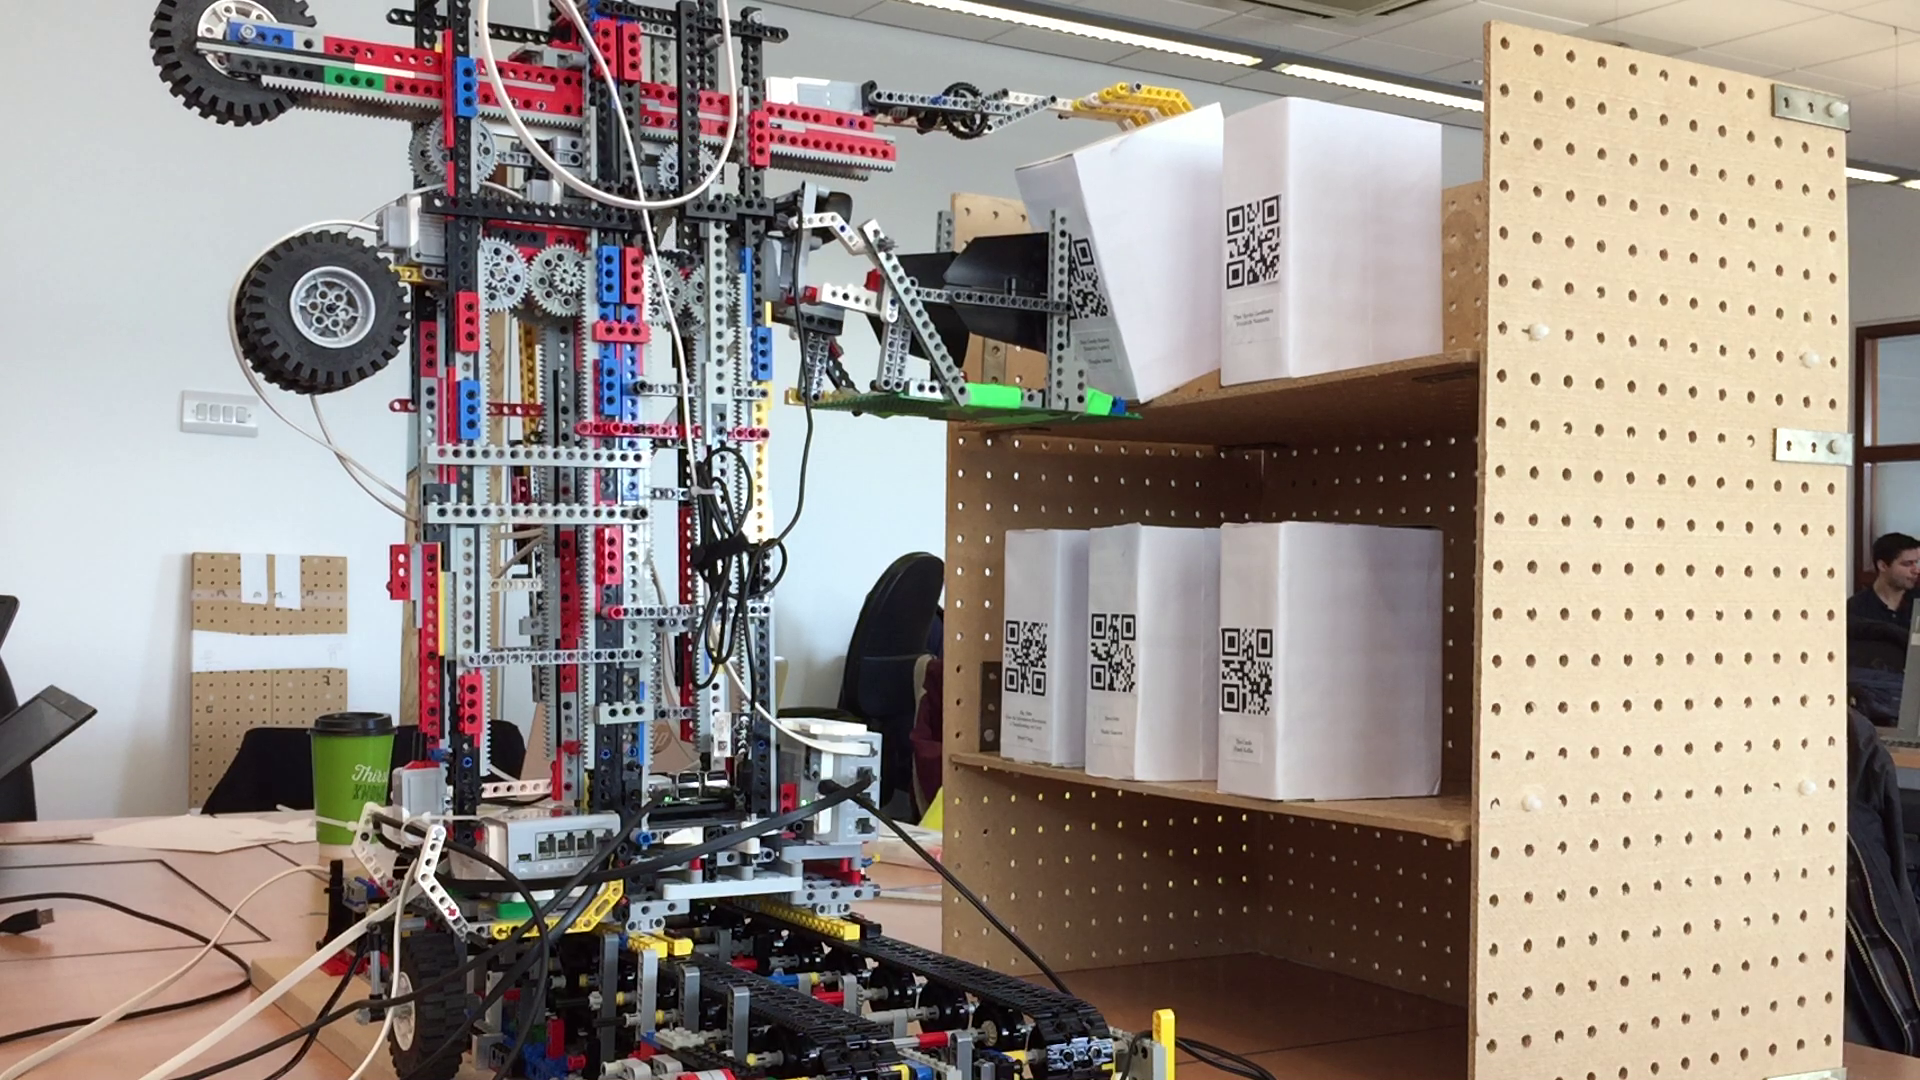
\includegraphics[width=\columnwidth]{figs/crane}}
\caption{Lego construction: highlight any salient features in the caption}
\label{fig:sample-fig}
\end{center}
\vskip -5mm
\end{figure} 


\subsection{Resource distribution}

The 200 hours per member will include the following for every member: {\bf at least} 15-20 hours worth of team meetings, 4 hours of demos with another 4 for preparation, 2 hours of workshops with each member attending at least one, and 1-2 hours for the individual reflection report. This leaves each member with 168 hours to dedicate to their work; roughly 500 hours per team. Each milestone has the same deadline across the teams - the date of the corresponding demo. They are shown in Table 2. Tables 3, 4, and 5 show the individual resource distribution for each of our three teams.
\begin{table}[]
  \begin{center}
  \begin{tabular}{ll}
    \hline
    Demo & Date   \\
    \hline
    1 & Feb 5 \\
    2 & Feb 26 \\
    3 & Mar 11 \\
    4 & Apr 1\\ \hline
  \end{tabular}
  \end{center}
  \caption{Demo dates.}
\end{table}

\begin{table*}[]
  \begin{center}
  \begin{small}
  \begin{tabular}{|c|l|l|l|c|}
    \hline
    {\bf Milestone} & {\bf Tasks} & {\bf Equipment} & {\bf Skills} & {\bf Est. Hours} \\ \hline
    1               & Build Lego bot & Lego & Lego building, Lego designing & 25 \\ \cline{2-5}
                    & Build Turtlebot & Turtlebot &  & 25 \\ \cline{2-5}
                    & Test and evaluate the two & - & Ability to evaluate from different metrics & 50 \\ \hline
    2               & Install arm & Turtlebot arm/Lego arm & Design Lego arm & 80 \\ \cline{2-5}
                    & Design and build scissor lift & Lego to build lift & Lego design/build & 60 \\ \cline{2-5}
                    & Design and build controls & Electronic components & Circuitry & 60 \\ \hline
    3               & Integrate camera to send to app & Camera, RasPi & Interfacing cam with software & 70 \\ \cline{2-5}
                    & Design 3D printed buttons & 3D print design tools & Ability to use said tools & 30 \\ \cline{2-5}
                    & Print and implement buttons & 3D printer & - & 20 \\ \hline
    4               & Tidy up of the aesthetic & - & Design, getting feedback & 50 \\ \cline{2-5}
                    & Maintainence & - & - & 30 \\ \hline
                    &                           &  & {\bf Total} & 500 \\ \hline
  \end{tabular}
  \end{small}
  \caption{{\bf Robot building team} resource distribution.}
  \end{center}
\end{table*}

\begin{table*}[]
  \begin{center}
  \begin{small}
  \begin{tabular}{|c|l|l|l|c|}
    \hline
    {\bf Milestone} & {\bf Tasks} & {\bf Equipment} & {\bf Skills} & {\bf Est. Hours} \\ \hline
    1               & Get robot moving & Access to robot & Ros (Turtlebot, Python (motors) & 60 \\ \cline{2-5}
                    & Get working with sensor input & Sensors & - & 25 \\ \hline
    2               & Using sensor input to stop & Sensor readings & Analysis & 120 \\ \cline{2-5}
                    & Using sensor input to detect environment & - & Real-time sensor analysis & 115 \\ \hline
    3               & Have lift working & - & Python for lift & 40 \\ \hline
    4               & Bot moves around to user defined paths/input & - & Sensor and/or camera analysis & 140 \\ \hline
                    &  &  & {\bf Total} & 500 \\ \hline
  \end{tabular}
  \end{small}
  \caption{{\bf Robot coding team} resource distribution.}
  \end{center}
\end{table*}

\begin{table*}[]
  \begin{center}
  \begin{small}
  \begin{tabular}{|c|l|l|l|c|}
    \hline
    {\bf Milestone} & {\bf Tasks} & {\bf Equipment} & {\bf Skills} & {\bf Est. Hours} \\ \hline
    1               & Set up app UI & Firebase & UI design, Android & 70 \\ \cline{2-5}
                    & Set up database system & Database management server & SQL(?) & 20 \\ \cline{2-5}
                    & Interface the database with the app & - & - & 30 \\ \hline
    2               & Set up robot control UI & - & - & 40 \\ \cline{2-5}
                    & Test UI & More UI testing required & - & 10 \\ \cline{2-5}
                    & Have app show alerts from bot & Information from robot & - & 40 \\ \hline
    3               & Implement calendar system & - & - & 40 \\ \cline{2-5}
                    & Add wake up alarm feature & - & - & 30 \\ \cline{2-5}
                    & Encryption of personal data & - & Network security & 60 \\ \cline{2-5}
                    & Receive photo from bot & Access to bot & - & 70 \\ \hline
    4               & App shows location of bot & Information from GPS tracker & - & 30 \\ \cline{2-5}
                    & App shows timetable/activity of bot & - & - & 30 \\ \cline{2-5}
                    & Final design of UI & Memory to store information & - & 30 \\ \hline
                    &                           &  & {\bf Total} & 500 \\ \hline
  \end{tabular}
  \end{small}
  \caption{{\bf App team} resource distribution.}
  \end{center}
\end{table*}


\subsection{Risk assessment} 

\underline{Robot building}

In terms of milestone 1, the main risk would be that the bot turned out to be infeasible as a design. We have decided to develop 2 prototypes as a contingency plan for this exact issue. This allows us to compare two designs and ultimately pick the one which we find to be a better choice.

For milestone 2, our team are planning to design and build a scissor lift from Lego. This should be fairly risk free. We also plan to build a hardware controller for the bot. At least one of these should be doable and whichever is not completed for this milestone can be worked on during the period of maintenance running up to the fourth demo.

This 30 hours of maintainence between milestone 3 and 4 will actually prevent mostly any risk that should arise with individual pieces of hardware, as it can be eaten into by the hardware team if need be.

\underline{Robot coding}

Having the robot move without the aid of a line on the ground is definitely a risk the robot coding team will have to keep in mind. It could prove to be more difficult than anticipated. The fact that sensors are not always 100\% accurate means that special care will have to be taken in the implementation of this.

Failure of a sensor could be catastrophic in a project where they are the centerpiece of the functionality. It is therefore of vital importance that we constantly check that they are all functioning as they should be.

The algorithms used by the robot will also be a challenge facing our robot coding team. We will make use of Traiko's help at this stage of development if the task proves to be more difficult than we anticipate.

\underline{App}

The use of Firebase should alleviate most of the risk in terms of the building of the app as it allows an easy way to get things off the ground. There are extensive resources to aid our developers in their progress should they hit a brick wall.

The UI will have to be usable for novice users and one of the risks is that this is not the case. The app team will use user testing in order to make sure they are putting out a usable product.


\section{Group organisation}
\begin{table}[]
  \begin{tabular}{lll}
    \hline
    Robot building & Robot coding & App development   \\
    \hline
    {\bf Jakub}          & {\bf Wojtek}       & {\bf Theo}              \\
    Luukas         & Ben          & Yuchen            \\
    Rebecca        & Errikos      & Ching Ling \\
    \hline
    Project management: & {\bf Michael} & \\
  \end{tabular}
  \caption{Team splits across the group. Names in bold are key points of contact.}
  \label{tab:group-split}
\end{table}

We will split the group into {\bf three core teams}: robot building, robot software, and app development (table~\ref{tab:group-split}). Each team has a team lead (in bold), responsible for co-ordinating with the other groups as necessary during the development process and holding responsibility for ensuring the group is tracking to its milestones.

The project manager (PM) holds overall responsibility for keeping the project on track: primarily through helping each team plan, execute, and validate its progress against milestones. The PM is also responsible for time management; writing up reports; and helping teams with any blockers they encounter in their work.

Structuring the teams in this manner allows us to use the {\it functional} organizational structure. This has particular benefits in allowing everyone within each team to focus on developing expertise in their area, as well as improving efficiency in communication within the team.

The disadvantage of using a functional structure is that it can make communication between teams difficult. To minimize this, we have decided a key point of contact (POC), in bold, for each team: POCs will communicate with each other and the PM on key issues and when cross-team collaboration is needed --- for example, in interfacing the robot hardware with the robot software. This eases communication between teams because it means there will only need to be four people meeting at once to represent all teams, rather than all ten group members needing to be present.

{\bf Each team will meet at a minimum once a week} to discuss their progress against their milestones. Work will be done in collaboration with the PM following an Agile approach: at each weekly meeting we will follow {\bf Plan, Develop, Review} methodology to iteratively update our approach and track our progress against our milestones.

In keeping with an Agile approach, {\bf team members will give daily updates on their work} (how they are progressing, if they have any blockers, and whether they need any help from other team members) in online `standups' on Slack. Additionally the team POCs will meet once a week to make sure that any cross-team integration issues are handled, as well as to support each other if needed. 

{\bf Code-sharing} will be done exclusively through GitHub. Using version control more generally allows us to track our work over time and easily deal with any merge conflicts or other issues that may come up in doing distributed development. GitHub was chosen primarily because all members of the group are somewhat familiar with it, meaning there will be a shallower learning curve to complete our project using it. 

Using GitHub also allows us to do {\bf task allocation and progress sharing} using GitHub projects. We will follow a Kanban approach, separating tasks into ``to do'', ``in progress'', and ``done'', with one board per team. Using Kanban allows for team members to clearly see what tasks need to be done before the next demo; choose to begin working on tasks they feel they are suitable for; and to identify where there may be blockers within their work (ie. cards that are spending extended time in ``to do''). Additionally, making these boards public allows for other teams to see how work is progressing in the rest of the group. Progress updates will also be discussed in weekly team meetings on a granular level and more broadly in POC meetings.

Additionally, in {\bf task allocation}, teams will decide the complexity of tasks by evaluating them using {\bf T-Shirt Sizing}, where the size or difficulty of each task is graded on a scale: XS, S, M, L, XL. This will allow team members to clearly see the estimated difficulty of each task and to assess where they need to dedicate their effort. 

{\bf Communication} will be done primarily through a dedicated Slack workspace, with separate channels for each team ({\tt robot-app}, {\tt robot-building}, {\tt robot-coding}, {\tt report-writing}, and {\tt general} for cross-team discussion). Using Slack allows us to integrate other apps, for example Doodle polls to decide group meeting times; and GitHub to track push or other notifications from our project repository. 


%% Include any references in a bibliography

\bibliography{plan-refs}

\end{document} 

